
\begin{figure}
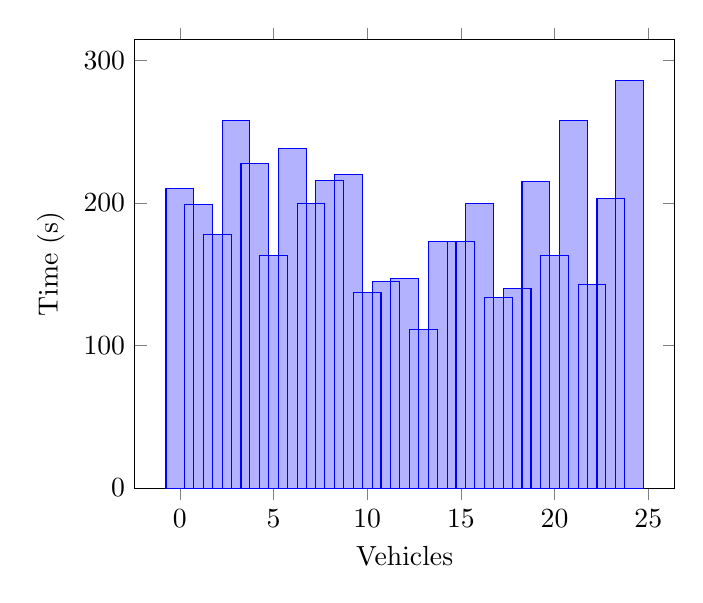
\begin{tikzpicture}
\begin{axis}[
legend style={anchor=west},
xlabel=Vehicles,
ylabel=Time (s),
ymin=0,
ybar,
]
\addplot coordinates {
(0, 210)
(1, 199)
(2, 178)
(3, 258)
(4, 228)
(5, 163)
(6, 238)
(7, 200)
(8, 216)
(9, 220)
(10, 137)
(11, 145)
(12, 147)
(13, 111)
(14, 173)
(15, 173)
(16, 200)
(17, 134)
(18, 140)
(19, 215)
(20, 163)
(21, 258)
(22, 143)
(23, 203)
(24, 286)
};

\end{axis}
\end{tikzpicture}
\label{tik:100:3_V, 3_V.-60, 4_S, 5_S, 5_S.-30, 7_S, 7_S.-25, 11_S, 11_S.-50, 13_S, 15_N, 17_S, 17_S.-60, 20_O, 21_O}
\caption{100 percent diving with GSC on route $3_V, 3_V.-60, 4_S, 5_S, 5_S.-30, 7_S, 7_S.-25, 11_S, 11_S.-50, 13_S, 15_N, 17_S, 17_S.-60, 20_O, 21_O$}
\end{figure}
